\documentclass[12pt,letterpaper,titlepage]{article}
\usepackage{fancyhdr}
\usepackage{fullpage}
\usepackage{lastpage}
\usepackage{graphicx}
\usepackage{verbatim}

\pdfpagewidth 8.5in
\pdfpageheight 11in
\textwidth 6.5in
\textheight 9in

%\pagestyle{fancyplain}
\pagestyle{fancy}
\lhead[]{Astrometry.net}
\chead[]{}
\rhead[]{Blind Solver: User Notes}
\cfoot[]{\thepage \ of \pageref{LastPage}}
\renewcommand{\headrulewidth}{0.5pt}
\renewcommand{\footrulewidth}{0pt}

\thispagestyle{empty}

\newcommand{\an}{Astrometry.net}
\newcommand{\code}[1]{\texttt{#1}}

\begin{document}
\title{Astrometry.net Blind Solver \\ User Notes}
\author{Dustin Lang}

\maketitle

\newpage

\section{Introduction}

This document is not meant to help you fix problems with building the \an{} code or 
running the basic \code{Makefile}.  These kinds of problems should be reported to the
mailing list.  Rather, this document is meant to help you take the next steps toward
using our code to solve your images.

%We will assume that you have downloaded and built the code and run it on the sample of
%SDSS fields we supplied.

-demo distribution

There are at least three distinct phases of ``the pipeline'' where you might want to
jump in.  For the purposes of this document, we'll start with the Astrometry.net catalog,
which is generated from the raw source catalogs: USNO-B and Tycho-2.  The
process of building the Astrometry.net catalog is deterministic and has no parameters.

\begin{figure}[h!]
\begin{center}
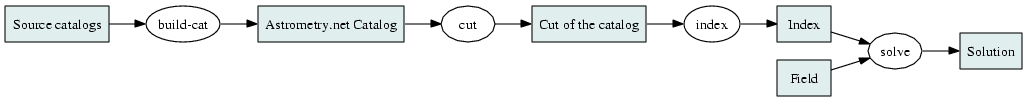
\includegraphics[width=\textwidth]{userdoc-fig-pipeline}
\caption{The blind solver pipeline, writ large.}
\label{fig-pipeline}
\end{center}
\end{figure}

The first major stage of the pipeline is \emph{making a cut}.  This involves selecting a 
spatially-uniform set of stars that is expected to be bright in the band or bands you are
interested in.  The two ``knobs'' of this process are determining which band you want to focus
on, and how spatially uniform you want the cut to be.  There is a trade-off between choosing bright
stars and ensuring that the chosen stars are spatially uniform.

The second major stage of the pipeline is \emph{building an index}.  This involves finding
``quads'': sets of four stars that satisfy particular local geometry constraints.  Again, there
is a tradeoff between building bright quads and ensuring that the quads are uniformly distributed.

The final stage of the pipeline is \emph{solving fields}.  The parameters in this stage tell the
solver where to find its inputs and where to put its output, how hard to work on each field
and how careful to be when deciding on a solution.

We'll go through the stages in reverse order (and ``degree of difficulty'').

\section{Solving}

-background: the solving process: fields (sorted in decreasing brightness),
 quads \& matching, (scale), agreement, verification.  Healpixes.  Fields
 (extensions within fields file); fieldids.

The solver program is called \code{slave} for historical reasons: at one point we envisioned
there being a \code{master} program that would plan how to solve a set of fields, and \code{slave}
workers that would carry out the plan.  In the end, it wasn't really necessary to have a \code{master}.

The \code{slave} program reads its parameters from a text file.  We typically generate a set of
input files by running a script, but if you are solving a few fields, it may just be easier to edit
the input file by hand.

In the demo distribution, the file \code{create-inputs-1} is a shell script that generates
input files for \code{slave}.  In the demo, it only writes one output file, \code{input.000}.
Its contents are shown below.

\begin{figure}[h!]
\begin{center}
\begin{tabular}{|@{\hspace{24pt}}c@{\hspace{24pt}}|}
\hline
\begin{minipage}{0.6\textwidth}
\vspace{10pt}
\begin{verbatim}
index ./sdss-1/sdss-1-02
field sdss-fields/sdssfield01-hp02.xy
fieldid 1
fields 0/2617
solved solved/solved.01
match match/match.00.01
done done/done.00.01
xcol X
ycol Y
sdepth 0
depth 60
cxdx_margin 0.05
parity 0
tol 0.004
fieldunits_lower 0.39
fieldunits_upper 0.41
agreetol 10
verify_dist 4
nagree_toverify 2
overlap_tosolve 0.25
overlap_tokeep 0.25
min_ninfield 50
do_correspond 0
threads 1
quiet
run
\end{verbatim}
\end{minipage}%
\\
\rule{0pt}{4pt} \\
\hline
\end{tabular}
\end{center}
\caption{Contents of \code{input.000} file: input file for \code{slave}.}
\label{input000}
\end{figure}

Let us briefly describe the various parameters.

\subsection{Required basic parameters}
\begin{description}
\item[\code{index <filename>}]: which index should be used.  The
  \code{slave} program will look for the files \code{<filename>.ckdt.fits},
  \code{<filename>.skdt.fits}, and \code{<filename>.quad.fits}.
\item[\code{field <filename>}]: file from which to read fields to solve.
  The program will look for the file \code{<filename>.fits}.
\item[\code{match <filename>}]: where to write the solutions.  This will be
  a FITS file containing a BINTABLE with many columns describing how the
  fields were solved.
\item[\code{depth <integer>}]: how many field objects to look at.
\item[\code{tol <real number>}] (default 0.01): how close in shape do quads
  have to be to be considered ``matching''.
\item[\code{run}]: run the solver with the parameters given.  This can be
  used to include multiple runs in one parameter file: list the first set
  of parameters, followed by \code{run}, then list the second set of
  parameters followed by \code{run}.  Note that all parameters are reset
  to their defaults after a \code{run} statement.
\item[\code{fields <int> [<int> ...] or <start-field>/<end-field>}]:
  either a list of field indices (starting with 0), or a range.\footnote{%
	You can also request that \code{slave} ask the \code{solvedserver} for a
	list of fields to try; see the \code{solvedserver} entry for details.}
\end{description}

\subsection{Parameters you almost certainly want to set}

\begin{description}
\item[\code{fieldunits\_lower <real>}]
\item[\code{fieldunits\_upper <real>}]: these two parameters tell the solver
  what your estimated (or known) pixel scale is, in arcseconds per pixel.
  This allows it to vastly narrow down the number of quads it has to check,
  which makes solving much much faster.  If you know the pixel scale exactly,
  you should set these bounds to perhaps a percent or two below and above
  the known value, in order to tolerate a bit of positional noise in the fields.
  In the demonstration, these parameters are set to $0.39$ and $0.41$,
  respectively.
\item[\code{verify\_dist <real>}]: setting this parameter enables verification,
  which you almost certainly want.  Recall that in the verification stage, the
  solver takes a potential match and projects each field object through the
  same transformation, then checks how many field objects overlap with
  indexed stars.  This parameter sets the maximum distance, in arcseconds,
  that a field object can be from an indexed star and still be considered
  to overlap.  You will want to set this value to be large enough to
  encompass the positional noise in the field objects and index stars, plus
  the error incurred by applying a transformation computed from correspondences
  between a small number of stars.  This value should also be at most half
  the \emph{deduplication distance} of the cut, though slight violations of
  this constraint won't cause huge problems.  In the demonstration, this
  parameter is set to $4$ arcseconds.
\item[\code{overlap\_tosolve <real>}]: when verification is enabled, this
  parameter tells the solver how good a solution has to be for it to stop
  trying further.  When a solution results in at least this fraction of
  field and index stars overlapping, the solver considers the field to be
  solved.  In the demonstration, it is set to $0.25$, though the majority of
  correct solutions have much larger overlap values.
\item[\code{overlap\_tokeep <real>}]: when verification is enabled, this
  parameter tells the solver how good a solution has to be in order for it
  to be recorded in the ``match'' file.  If you set it to a value smaller
  than \code{overlap\_tosolve}, then the solver will record the potential
  solution but continue to search further.  This is useful if you are
  exploring the ROC curve (false positive vs false negative rate); you can
  run the solver once, then use the program \code{agreeable} to see what
  would have happened if you had set \code{overlap\_tosolve} lower.
  In the demonstration this parameter is set to $0.25$.  Unless you are
  exploring the ROC curve, you probably want to set it to the same value as
  \code{overlap\_tosolve}.
\item[\code{min\_ninfield <int>}]: when verification is enabled, this parameter
  sets a minimum on the number of index stars that are contained in a
  potential field location.  This is to prevent the case where a quad matches
  a nearly empty region of the index, but a few field objects happen to overlap
  with indexed stars, yielding a high \code{overlap} score.  This parameter sets
  a minimum on the ``denominator'' of the \code{overlap} fraction.  That is,
  when the bounds of the field are projected into the index, the index must
  contain at least this number of stars or the match is rejected.  In the
  demonstration this parameter is set to $50$.  You will probably want to set
  it by computing the expected density of index stars in a field and taking
  half or a third this value.
\item[\code{nagree\_toverify <int>}]: this parameter determines how many
  matches must \emph{agree} before the \emph{verification} process is run on
  the matches.  This is useful because the verification process is relatively
  expensive, so it can be useful to accumulate more evidence before testing
  hypotheses.  The tradeoff is that if a field contains fewer than this number
  of matches, then the correct match will never be tested and the field will
  not be solved.  In the demonstration, this value is set to $2$.  In our
  experiments we typically do a ``quick'' run with a setting of $2$, then a
  more thorough run with a setting of $1$.  There is probably no point setting
  this parameter to any value other than $1$ or $2$.
\item[\code{agreetol <real>}]: this determines how close a pair of matches
  must be to be considered ``in agreement''.
  %It is specified as the RMS distance
  %in arcseconds between the corners of the field proposed by the two matches.
  %That is, 
  We project the bottom-left and upper-right corner of the field 
  onto the celestial sphere according
  to the projections implied by the two matches,
  and measure the RMS distance them, in arcseconds.
\end{description}







\begin{description}
\item[\code{firstfield <int>} and \code{lastfield <int>}]: used in conjunction
  with the \code{solvedserver} option: ask the \code{solvedserver} which fields
  to try, in the range from \code{firstfield} to \code{lastfield}.
\end{description}

\subsection{Optional parameters}
\begin{description}
\item[\code{quiet}]
\item[\code{maxquads <int>}]
\item[\code{cxdx\_margin <real>}]
\item[\code{do\_correspond <0/1>}] (default 1)
\item[\code{xcol <string>}] (default \code{X})
\item[\code{ycol <string>}] (default \code{Y})
\item[\code{fieldid <int>}]
\item[\code{done <filename>}]
\item[\code{solved <filename>}]
\item[\code{solvedserver <hostname:port>}]
\item[\code{firstfield <int>}]
\item[\code{lastfield <int>}]
\item[\code{fields <int>}]
\item[\code{sdepth <int>}] (default 0)
\item[\code{parity <0/1>}] (default 0)
\item[\code{threads <int>}]
\end{description}

\section{Indexing}

\section{Cutting}

\end{document}
